\marginnote{Beginning of using\_em.tex}

For all the experiments in this section, we build different grammars
from the example curve in Figure \ref{fig-romer-example}. We then
retrain the grammar in various ways using the training set shown in
Figure \ref{fig-romer-train}. We show samples from each model in order
to demonstrate what has been learned. We want models to generate
reasonable-looking human silhouettes, and ideally generate some that
differ significantly from any training example. For instance, we would
like the model to learn that limbs can move independently of one
another.

\begin{figure}

\includegraphics[width=\linewidth]{experiments/3.learning/simple_tuning/output.d/examples.png}
\caption{The example curve, from which we build a grammar with hand-chosen rules.}
\label{fig-romer-example}
\end{figure}

\begin{figure}
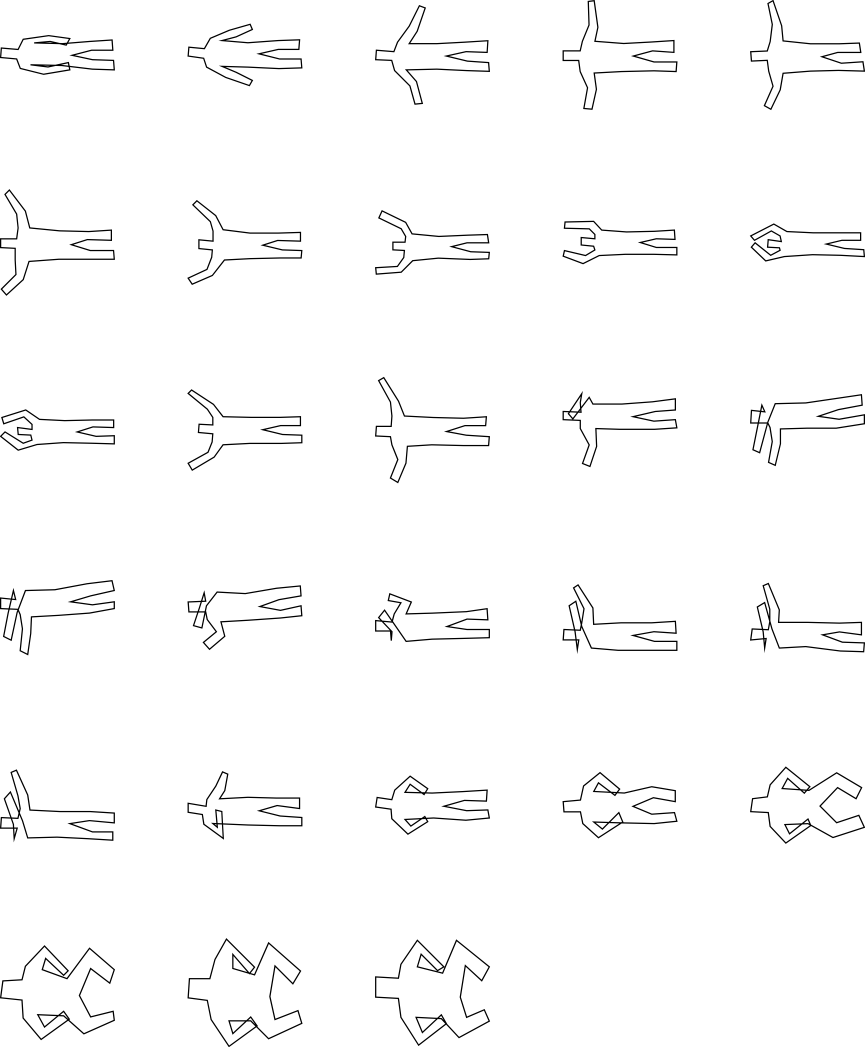
\includegraphics[width=4in]{experiments/3.learning/simple_tuning/output.d/training.png}
\caption{Training set}
\label{fig-romer-train}
\end{figure}

\subsection{Simple tuning of hand-built grammar with curves of constant length}

First, we use EM to train an initial grammar that has no choices. Our
grammar is produced from a hand-chosen decomposition. Samples from the
grammar after two rounds of training are shown in Figure
\ref{fig-em-simple}. Since we are using unimodal midpoint
distributions, and our grammar has no choice, all the samples are
slight variations on one particular mean shape. The mean shape chosen
is a very reasonable one, although the arms are longer than is ideal.

\begin{figure}
\includegraphics[width=6in]{experiments/3.learning/simple_tuning/output.d/gram.2.d/samples.png}
\caption{Simple tuning of hand-built grammar with curves of constant length}
\label{fig-em-simple}
\end{figure}

\subsection{Tuning with multiple midpoints, and curves of constant length}

In the next experiment, we enrich the grammar by adding in several
copies (in this case, five) of each rule, with jittered midpoints. (If
we used the same midpoint for each copy of the rule, parses could use
the rules interchangeably, and EM would never break this symmetry.)
Figure \ref{fig-em-multi} shows samples from the grammar after ten
rounds of training. The samples show significantly more variation than
in the previous experiment, but they also include many ill-formed and
unlikely shapes. This is because the grammar cannot model correlations
between levels, so that e.g., it cannot pick the location of the elbow
based on the location of the hand, which means that the arm is often
ill-formed and self-intersecting.

\begin{figure}
\includegraphics[width=6in]{experiments/3.learning/multi_tuning/output.d/gram.10.d/samples.png}
\caption{Tuning with multiple midpoints, and curves of constant length}
\label{fig-em-multi}
\end{figure}

\subsection{Tuning with multiple midpoints, learning multi-level correlations}

In this experiment, we enrich the grammar by adding in several copies
of each nonterminal, each of which has several copies of the original
rule with jittered midpoints. If our original rule was $X\to YZ$, then
we have five copies each of $X,Y,Z$, and each $X_i$ has five rules of
the form $X_i \to Y_j Z_k$, where $j$ and $k$ are chosen independently
at random.

Figure \ref{fig-em-correlated} shows samples from the grammar after
ten rounds of training. The silhouettes look much better than in the
previous experiment. This is because we have learned correlations
between levels, i.e., the choice of rule at a higher level influences
the choice of rule at a lower level.

\begin{figure}
\includegraphics[width=6in]{experiments/3.learning/correlated_tuning/output.d/gram.10.d/samples.png}
\caption{Tuning with multiple midpoints, learning multi-level correlations}
\label{fig-em-correlated}
\end{figure}

\subsection{Multi-level correlations, carefully-chosen sdf}

This experiment is the same as the previous experiment, but the
decomposition of the curve has been chosen more carefully. (I think it
is the optimal decomposition found in Chapter \ref{chap-structure}.)
Samples from the grammar after ten rounds of training are seen in
Figure \ref{fig-em-sdf}. The samples look slightly better than in the
previous experiment. This shows that learning depends on the initial
choice of model structure.

\begin{figure}
\includegraphics[width=6in]{experiments/3.learning/sdf_tuning/output.d/gram.10.d/samples.png}
\caption{Multi-level correlations, carefully-chosen sdf}
\label{fig-em-sdf}
\end{figure}

\subsection{Adding in multiple midpoints as needed}

In this experiment, we enrich the grammar by adding new rules during
each round of training. Specifically, during each round, we identify
the five most expensive uses of a binary rules in a Viterbi parse. If
one such is $X\to YZ$, we add new symbols $X',Y',Z'$, duplicate all
rules involving any of $X,Y,Z$, and then add a new rule $X'\to Y'Z'$
whose midpoint distribution is centered around the midpoint used in
the Viterbi parse. We then do five sub-rounds of EM tuning.

Samples from the grammar are shown in Figure \ref{fig-em-incremental}
after 19, 20, and 30 rounds of training.

\begin{figure}
\includegraphics[width=6in]{experiments/3.learning/incremental/output.d/gram.19.d/samples.png}
\includegraphics[width=6in]{experiments/3.learning/incremental/output.d/gram.20.d/samples.png}
\includegraphics[width=6in]{experiments/3.learning/incremental/output.d/gram.30.d/samples.png}
\caption{Adding in multiple midpoints as needed}
\label{fig-em-incremental}
\end{figure}

\subsection{Training with full grammar}

In this experiment, we build a grammar from the example curve that
allows all possible decompositions, and then train using EM. In Figure
\ref{fig-em-full}, we show samples from the grammar after five and ten
rounds of training.

\begin{figure}
\includegraphics[width=6in]{output/3.learning/full_tuning/gram.5.d/samples.png}
\includegraphics[width=6in]{output/3.learning/full_tuning/gram.10.d/samples.png}
\caption{Training with full grammar}
\label{fig-em-full}
\end{figure}


\marginnote{End of using\_em.tex}
